\documentclass[a4paper]{article}

\usepackage[english]{babel}
\usepackage[utf8x]{inputenc}
\usepackage{graphicx}
\usepackage[colorinlistoftodos]{todonotes}
\usepackage{tabularx}
\usepackage{amsmath}
\usepackage{amssymb}
\usepackage{amsfonts}
\usepackage{adjustbox,lipsum}
\usepackage{fullpage}
\usepackage{times}
\usepackage{fancyhdr,graphicx,amsmath,amssymb}
\usepackage[ruled,vlined]{algorithm2e}


\title{Distributed SNN Clustering for large document collections}

\newcommand{\set}[1]{\mathcal{#1}}
\newcommand*\pct{\scalebox{.9}{\%}}

\SetKwInput{KwData}{Input}
\SetKwInput{KwResult}{Output}

\begin{document}
\maketitle

\begin{abstract}
Your abstract.
\end{abstract}

\section{Introduction}
As a consequence of the explosive growth of the WEB, the integration of search engines such as Google into personal computers and mobile devices, and the wide use of social networks, the task of clustering text data, i.e. Tweets or documents in a search engine, has each time an increasing importance because of the necessity of unraveling the underlying categories in large volumes of text data. Nowadays the generation of large amounts of documents surpasses the computational power of personal computers and even of high performance computers.
As an example, it is estimated that the amount of WEB pages that popular search engines such as Yahoo! and Google index is higher than the tens of a billion \cite{www}.
It is therefore of great interest to develop algorithmic techniques capable of automatically organize, classify and summarize document collections distributed in multiple machines of a network, and that also perform efficiently in modern hardware, particularly within parallel processing frameworks in multi-core architectures. In real problems such as \textit{Collection Selection} for distributed document databases, in which for a given query the computer node containing the most suitable sub-collection must be selected to answer it \cite{CM13}, the challenges related to the scalability and efficiency of \textit{Knowledge Discovery} methods have become very important. Traditional algorithms often assume that the whole dataset is loaded into main memory (RAM) and thus every document can be accessed at any time with no access latency. In scenarios where the size of the collection is much bigger than the amount of available RAM either because of the number of documents or the length of each document, this ideal loading process is unfeasible due to real constraints in the storage or computational capabilities.


Often, text data is structured in digital collections of documents whose length (number of characters) is variable, e.g. WEB pages or the content generated by users in social networks such as Twitter or Facebook. In order to enable the processing of these collections, in a first stage of preprocessing a set of words occurring in the documents are extracted and sorted in lexicographical order; this word set is referred to as the Vocabulary. Then, the content of every document in the collection is represented as a vector in which each dimension denotes a specific word of the Vocabulary and its value in a document vector is given by a function of the number of occurrences of the word within the document and the number of documents in which it appears. As a natural consequence of the lexical richness of every language, the size of the Vocabulary, and in turn the dimensionality of the vector space onto which a document is represented,  is far bigger than the data size that traditional clustering algorithms manage. Because of this, the task of automatic document clustering has high computational and storage (RAM and secondary memory) costs. Along with this, when the number of documents is large (tens or hundreds of thousand and even millions of items) then traditional techniques for processing and clustering documents, and current computational capabilities of a single machine and also high performance machines are insufficient. Even in the most favorable scenario the storage and computational power tackle the challenge but the response time are excessive.


There exist three approaches successfully applied to the construction of clustering algorithms capable of processing large volumes of data. The first one introduces constraints on the number of passes allowed on a document (related to the amount of time it is loaded into main memory)[CITA]. The second one exploits current multi-core architectures to perform parallel processing of the data, which does not solve the massive volume problem [CITA]. The last one combines the computational power of a single machine together with the scalable storage capability of a distributed system by partitioning the dataset into several independent machines connected through a network[CITA].


The last above mentioned approach seems promising since it allows to exploit the local capabilities of single computers with multi-core architectures without sacrificing scalability to large data volumes because of its distributed design. Within this path there are two contexts regarding the data generation scenario. On the one hand, in some problems where the dataset is large but collected in a centralized fashion, the strategy employed consists in partitioning the collection into several machines or nodes of a network. This scheme leads to the transmission of a lot of data during the execution of the algorithm \cite{N15}. On the other hand, there are some problems where the data is generated in a distributed fashion and where besides it is not feasible to centralize the data because of high transmission costs or privacy issues \cite{JW05,LHLX12}, e.g. search engines work with document collections originated and stored in different geographical locations.
%\subsection*{Outline}

This document is structured as follows: First, a review of the literature on scalable and distributed data clustering methods is presented. Next, the proposed method is shown. Finally,the experimental design along with the attained results and the final remarks are presented. 

\section{Distributed Clustering Algorithms}
As far as we know from the literature, most of the existing efforts for the construction of clustering techniques capable of operating in scenarios where the data is distributed have been focused on low dimensional data (less than 100 attributes) in contrast with document datasets in which a document vector for a small collection may have about $10^4$ attributes. Nevertheless, the main advances in distributed data clustering are detailed below, specially highlighting those contributions focused on methods capable of dealing with high dimensional data.

\subsection{Main contributions on parallel algorithms}
\cite{XJK99} and \cite{DM99} propose parallel extensions for the algorithms DBSCAN and K-Means. Another scalable approach based on secondary memory consists in designing algorithms capable of working within the MapReduce framework\footnote{Hadoop MapReduce is a software solution that enables the construction of applications capable of processing large amounts of data (e.g. Terabytes) in a parallel fashion over big computer clusters.}. In this context it is possible to highlight the contributions made by \cite{DDGR07} in which they propose an implementation of the EM algorithm and also by \cite{EIM11} in which they tackle the K-Median problem by using MapReduce. Another parallel approach for K-Means is presented by \cite{BMVKV12} and it is called K-Means$++$. Additionally, the EM-Tree proposed by \cite{VVGN15} is very interesting since it allows to process very large datasets, specifically the authors show that it can handle hundred of millions of WEB pages.

\subsection{Approaches capable of dealing with high dimensional data} 
\cite{KHSJ01} propose a method to obtain the Principal Components (PCA) over heterogeneous and distributed data. Based on this contribution on dimensionality reduction they also propose a clustering method that works over high dimensional data. Once the global principal components are obtained by using the distributed method and transmitted to each node, local data are projected onto the components and then a traditional clustering technique is applied. Finally, a central node integrates the local clusters in order to obtain a global clustering model.

Several years later, \cite{LBK13} present another algorithm for principal components extraction over distributed data. To this end, each node computes PCA over its local data and transmit a fraction of them to a central node. This node uses the received components to estimate the global principal components, which are later transmitted to each node. After this, in every node, local data are projected onto the global components and the projected data are used for computing a coreset by means of a distributed algorithm. The global coreset built from the local projected data will be finally used to obtain a global clustering model.  

\cite{LZO03} propose an algorithm called D-CoFD for high dimensional and distributed data that also is capable of dealing with homogeneous and heterogeneous environments.


\subsection{Density based approaches}
\cite{JKP03} propose a distributed data clustering technique in which local nodes build models and transmit a set of representatives of each cluster to a central node. In this node a centralized clustering method is applied over the representatives and then the resulting model is re-transmitted to the local nodes to update their models.

\cite{KLM03} propose a clustering technique based on density estimates.

\cite{JKP04} present a scalable version of DBSCAN that is also capable of operating over distributed collections. First, the best local representatives a selected depending on the number of points that each one represents and then those chosen points are sent to a central node. This central node clusters the received local representatives into a single new model, which is re-transmitted to the other nodes so they can improve their local group structure.


\subsection{Approaches based on parametric models}
\cite{MG03} propose a clustering method that combines local parametric models, each one built on a single node, into a general one. The main contribution of this work consists in a method capable of dealing with distributed data that also considers the privacy of the local data in each node, since it transmits a summary of each local data and not raw points.

\cite{KKPS05} present a technique that fits a Gaussian mixture model in each node using the EM algorithm. Finally, all these Gaussian mixture models are integrated into a general parametric model.


\subsection{Approaches based on representative points}

\cite{FZ00} extend centroid based techniques to identify groups over distributed data. Specifically, they extend K-Means, K-Harmonic-Means and EM.

\cite{ZLW08} propose an approximate K-Median clustering technique that works over stresaming data, i.e. data is continuously collected. 

\cite{BEL13} address the distributed clustering problem by using centroid based techniques that use a novel coreset construction method that works for distributed data.

\cite{NC14} tackle the problem of the parameter selection of the K-Means clustering algorithm by using evolutionary algorithms. Additionally, they propose two strategies inspired in evolutionary algorithms for clustering distributed data using centroids. 

\subsection{Hierarchical clustering approaches}

A hierarchical algorithm that works on distributed and heterogeneous data is presented by \cite{JK00}. This method assumes that data is vertically partitioned, thus all nodes contain the same set of points, but characterized by different features. At the beginning, a dendrogram is generated in each node, and then it is transmitted to a central node. Finally, this node combines all the dendrograms into a global model.  


\cite{JCHAC15} propose a hierarchical clustering algorithm for distributed data that builds the clusters by incrementally processing the data points. The authors re-state the hierarchical clustering problem as a Minimum Spanning Tree construction problem over a graph. In order to integrate several local models they also propose a technique for combining multiple minimum spanning trees, assuming that these trees were obtained from disjoint subgraphs of the complete original graph. This mixture procedure iterates until a single tree is obtained, which in turn denotes the hierarchical clustering originally pursued. 

\section{Proposal}
% Clustering can be used to reduce the amount of data and to induce a categorization
%The goal of clustering is to reduce the amount of data by categorizing or grouping similar data items together
% Illustrate the structure of a given dataset
In this work we present a distributed clustering algorithm based on \textit{Shared-Nearest-Neighbor} (SNN) clustering. This method automatically identifies the number of  underlying groups along with a set of representative points for each one.
We pose that this method is able to deal with collections arbitrarily distributed across a Master/Worker architecture as depicted in figure \ref{fig:distributed_architecture} and the overall algorithm operates in two stages: The first one starts when the data is randomly partitioned and distributed into several nodes, then each one generates a set of representative points per cluster, i.e. \textit{core-points}, and finally, transmits back a sample set of these \textit{core-points} to the master node. In the second stage, the central node joins the sample points received and then starts a centralized SNN clustering over them. Finally, the set of representative points is labeled and also a new set of \textit{core-points} that summarizes the overall collection is obtained.  

\begin{figure}[h]
\centering
  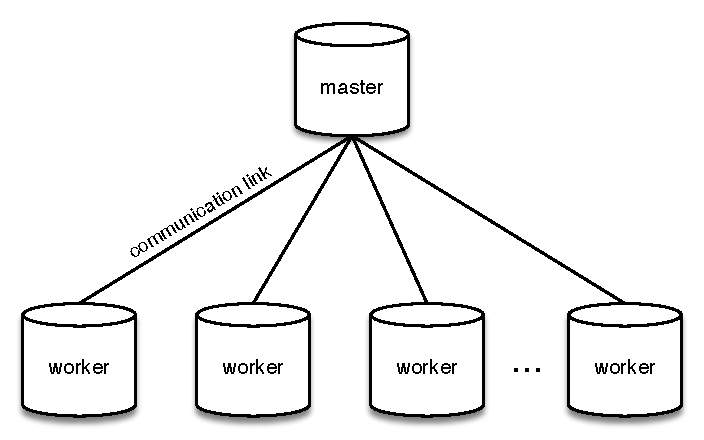
\includegraphics[scale=0.8]{distributed_architecture.pdf}
  \caption{Network architecture employed by the proposed algorithm}
  \label{fig:distributed_architecture}
\end{figure}


%about the parameters
\subsection*{Parameters of the algorithm}
The proposed method comprehends three parameters, namely $k$, $\mathsf{Eps}$, $\mathsf{MinPts}$ and $\omega$. The value of parameter $k$ determines the size of the neighborhood over which the SNN similarity measure is going to be computed. In the SNN space, the value of $\mathsf{Eps}$ denotes the similarity threshold beyond which two points are considered as close. Additionally, a point is identified as a \textit{core-point} when the number of points close to it in the SNN space surpasses the value of parameter $\mathsf{MinPts}$. Finally, the value of the  parameter $\omega$ rules the size of the sample set of \textit{core-points} that is going to be transmitted.

\subsection*{Initial stage}
The method starts by randomly partitioning and distributing the dataset into several worker nodes.
In this primary stage, after a worker node $n_i$ receives its data chunk $\mathcal{D}_i$, it starts to identify the core-points by following algorithm $\mathsf{SnnCorePoints}$ described in algorithm \ref{alg:snncorepointid}. 
Once its core-point set $\mathcal{C}_i$ is built, an attempt to label each point $p\in \mathcal{C}_i$ is performed. That is, when the similarity value between $p$ and its closest core-point $q$ is higher than the value of parameter $\mathsf{Eps}$, then the same label of $q$ is assigned to $p$. Otherwise, $p$ is tagged by a new label, i.e. it represents a new cluster.
Regarding the labeled core-points, a weighted sample from each group is drawn. The weight of a point  follows the expression:\[\dfrac{1 - ( N_l/N_c ) }{2\cdot N_l}\] where $N_c$ denotes the number of labeled core-points and $N_l$ the number of points labeled with label $l$. The expression shown above denotes that the sampling weight of a core-point is inverse to its group size as it is depicted in figure \ref{fig:group_weight}.
The overall procedure is described in algorithm \ref{alg:coresample}. 

\begin{figure}[h]
  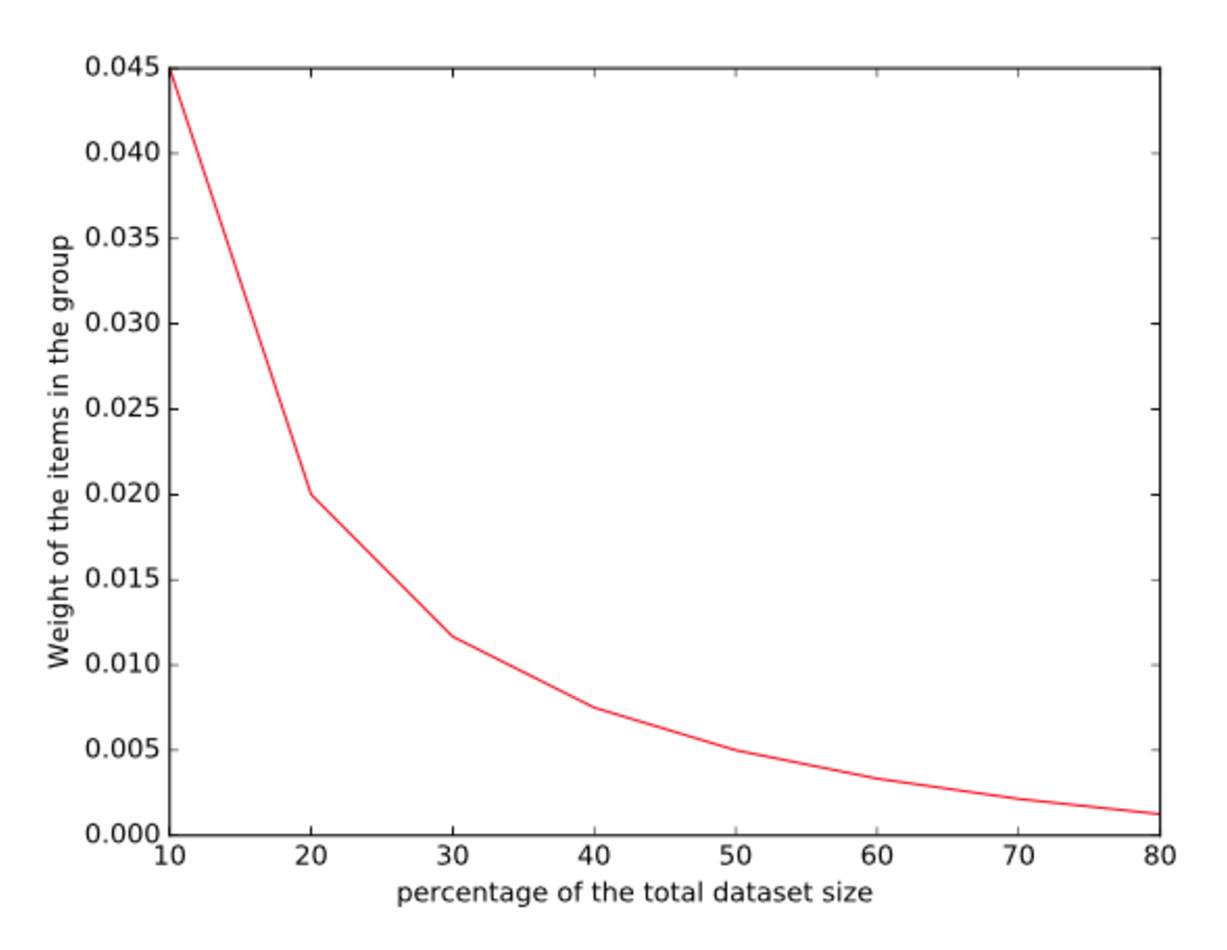
\includegraphics[width=\linewidth]{group_weights.pdf}
  \caption{Weight of each item in a group vs the relative size of the group in comparison with the total dataset size.}
  \label{fig:group_weight}
\end{figure}



%\subsubsection*{Identification of core-points}
% TODO: no se que poner aqui aun!!
\subsection*{Final stage}
See algorithm \ref{alg:centralproc}

%algorithms
\begin{algorithm}[H]
   \DontPrintSemicolon
  \SetKwFunction{snncpts}{SnnCorePoints}
  \SetKwProg{Fn}{Function}{:}{}
  
  \Fn{\snncpts{$\mathcal{D}$, $k$, $\mathsf{Eps}$, $\mathsf{MinPts}$}}{
  \ForEach{$p\in\mathcal{D}$}{compute $KNN_{k}(p)$\;}
  \ForEach{$p\in \mathcal{D}$}{
  	\ForEach{$q\neq p\in \mathcal{D}$}{
		$\mathsf{SNN}_{k}(p,q)\leftarrow \#(KNN_{k}(p)\cap KNN_{k}(q))$\; 
    }
    $\mathsf{density}(p)\leftarrow \#\{q\neq p\in\mathcal{D} |\mathsf{SNN}_{k}(p,q)>\mathsf{Eps}\}$\;
    \lIf{$\mathsf{density}(p)>\mathsf{MinPts}$}{Mark $p$ as \textbf{core-point}}
  }
$\mathcal{C}\leftarrow$ all points marked as  \textbf{core-point}\;
\KwRet $\mathcal{C}$ , $\mathsf{SNN}_{k}$\;
  }
  \label{alg:snncorepointid}
\caption{Identification of core-points from a dataset}
\end{algorithm}

%node
\begin{algorithm}[H]
% \KwData{$\mathcal{D}$ denotes the local subset of the data, $k$, $\mathsf{Eps}$, $\mathsf{MinPts}$, $\omega\in [0,1]$}
% \KwResult{List of representative points per group}
 \DontPrintSemicolon
  \SetKwFunction{sampleld}{SampleLocalData}
  \SetKwProg{Fn}{Function}{:}{}
  
  \Fn{\sampleld{$\mathcal{D}$, $k$, $\mathsf{Eps}$, $\mathsf{MinPts}$, $\omega\in [0,1]$}}{
  
  $\mathcal{C},\mathsf{SNN}_k\leftarrow$ \snncpts{$\mathcal{D}$, $k$, $\mathsf{Eps}$, $\mathsf{MinPts}$}\;
  
 \ForEach{\bf{core-point} $p\in \mathcal{C}$}{
 	\If{$p$ is not visited}{
    	Assign a new cluster label $l_p$ to $p$\;
	mark $p$ as visited\;
    	\ForEach{Not visited $q\neq p\in\mathcal{C}$}{
        	\If{$\mathsf{SNN}_{k}(p,q)>\mathsf{Eps}$}{
            	Assign label $l_p$ to $q$\;
		mark $q$ as visited\;
            }
    	}
    }    
}
 $N_c\leftarrow$Number of labeled \bf{core-points}\;
 $S\leftarrow\emptyset$\;
 \ForEach{cluster $l$ having size $N_l$}{
 	$S\leftarrow$ Add $\omega\cdot N_l$ points sampled from group $l$ with weight $\dfrac{1 - ( N_l/N_c ) }{2\cdot N_l}$\;
 }
 \KwRet sampled data $S$\;%en L124 se ejecuta el cludtering sobre los datos centralizados.
 }
 \label{alg:coresample}
\caption{Selection of representative points executed in a node}
\end{algorithm}

%central
\begin{algorithm}[H]
 \DontPrintSemicolon
\SetFillComment
\SetKwFor{ForEach}{On each}{execute}{endfch}
\KwData{$\mathcal{D}$ denotes the local subset of the data, $k$, $\mathsf{Eps}$, $\mathsf{MinPts}$, $\omega\in [0,1]$}
%\KwResult{List of representative points per group}
Partition the dataset $\mathcal{D}$ into $M$ subsets $\{D_1, D_2, \ldots D_M\}$\;
\ForEach{node $n_i$}{
	$S_i\leftarrow$ \sampleld{$D_i$}\tcc{remote procedure call on node $m_i$}
}
$S\leftarrow [S_1,S_2,\ldots S_M]$\;
$\mathcal{C},\mathsf{SNN}_k\leftarrow$ \snncpts{$\mathcal{S}$, $k$, $\mathsf{Eps}$, $\mathsf{MinPts}$}\;
\SetKwFor{ForEach}{foreach}{do}{endfch}
 \ForEach{\bf{core-point} $p\in \mathcal{C}$}{
 	\If{$p$ is not visited}{
    	Assign a new cluster label $l_p$ to $p$\;
	mark $p$ as visited\;
    	\ForEach{Not visited $q\neq p\in\mathcal{C}$}{
        		\If{$\mathsf{SNN}_{k}(p,q)>\mathsf{Eps}$}{
        	    		Assign label $l_p$ to $q$\;
			mark $q$ as visited
        		}
    	}
    }    
}

\ForEach{p $\in S\setminus \mathcal{C}$}{
	$n_p\leftarrow \operatorname*{arg\,max}_{q\in \mathcal{C}} \mathsf{SNN}_{k}(p,q)$\;
	\lIf{$\mathsf{SNN}_{k}(p,n_p)<\mathsf{Eps}$}{
		Mark $p$ as \textbf{noise}
	}
	\lElse{
		Assign label $l_{n_q}$ to $p$
	}
}
%Labeled points in $\mathcal{S} Final set of points\;
\KwResult{$\{p\in S\ |\ \exists\ l_p\}$}
  \label{alg:centralproc}
\caption{Procedure executed by the master node to generate the list of representative points per group}
\end{algorithm}


%TOYEXAMPLE
\begin{figure}[hp]
\centering
  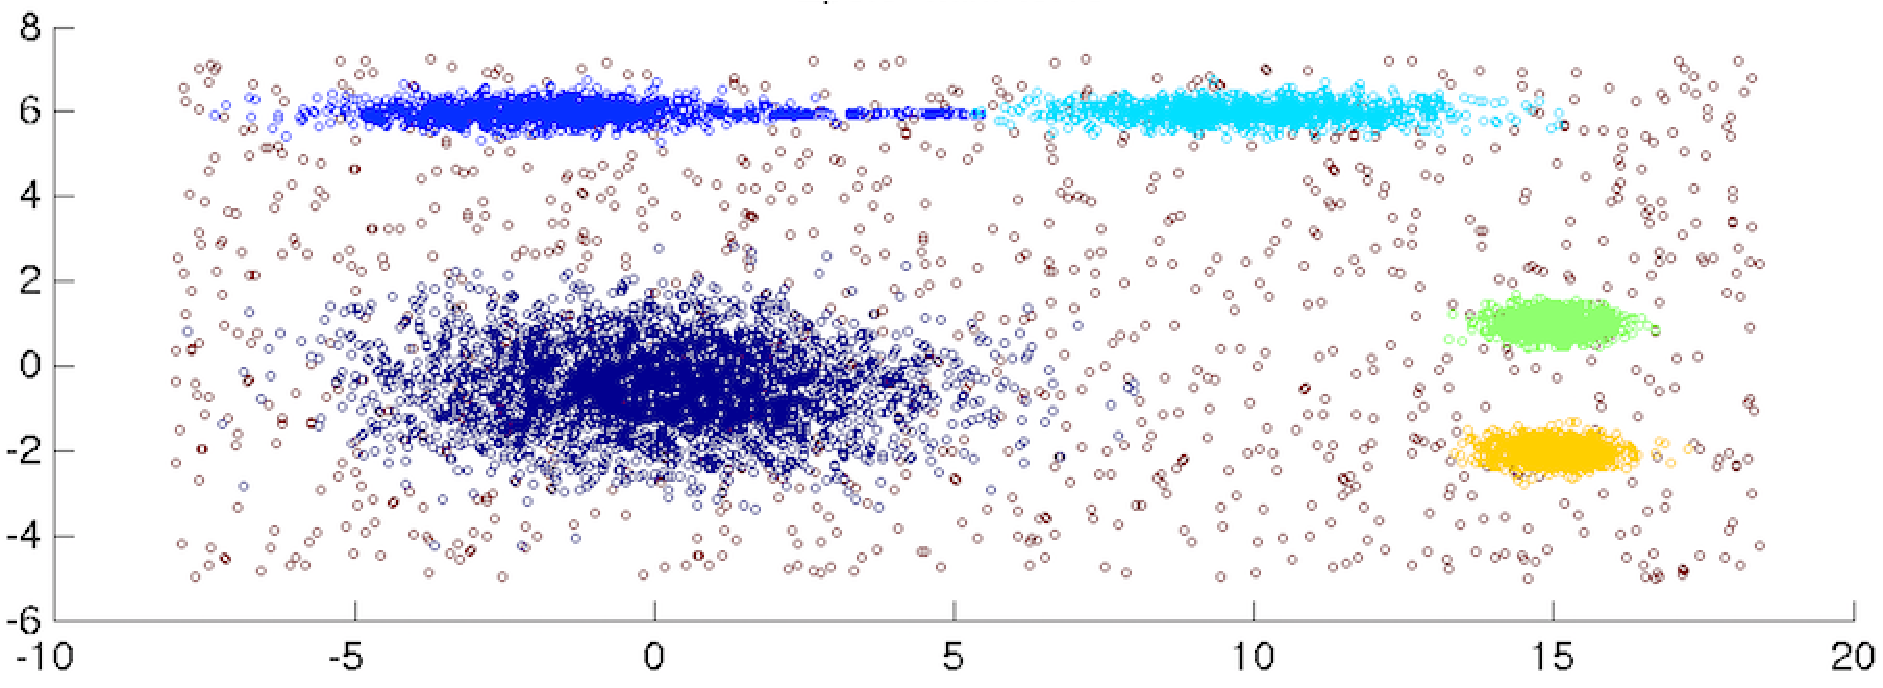
\includegraphics[scale=0.45]
  {toy_example_original.pdf}
  \caption{Toy example: Original data.}
  \label{fig:toy_original}
\end{figure}

\begin{figure}[hp]
\centering
  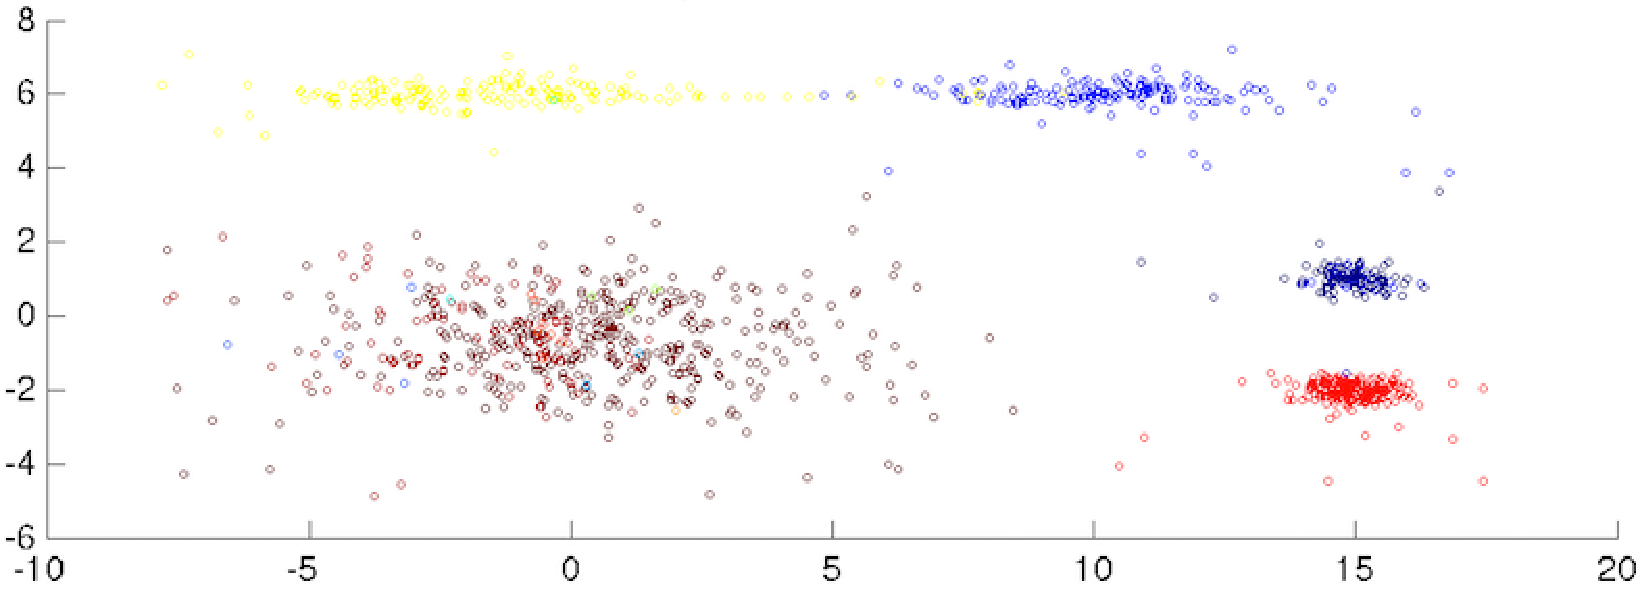
\includegraphics[scale=0.5]{toy_example_after_Dsnn_2.pdf}
  \caption{Toy example: Data after distributed snn clustering with $Eps=50$.}
  \label{fig:toy_dsnn1}
\end{figure}

\begin{figure}[hp]
\centering
  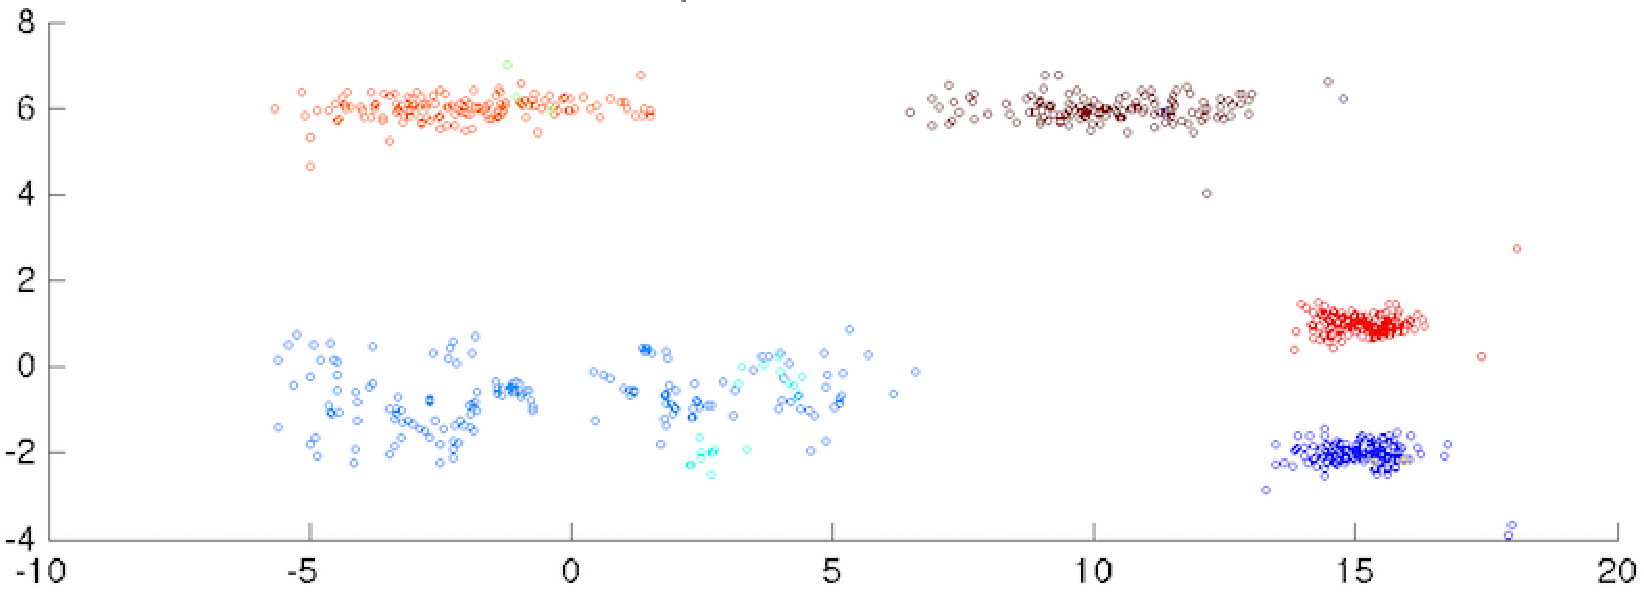
\includegraphics[scale=0.5]{toy_example_after_Dsnn_1.pdf}
  \caption{Toy example: Data after distributed snn clustering with $Eps=60$.}
  \label{fig:toy_dsnn2}
\end{figure}



\section{Experimental design and results}
\begin{table}[h]
\centering
\noindent\adjustbox{max width=\textwidth}{%
\begin{tabular}{llrrrc}
    \hline
    Dataset & Description &instances & $|\set{V}|$ & classes & $\pct$NNZ\\ \hline
\textit{20NG} & 20-newsgroup data, m5 partition. & $4743 $ & $41223$ & $5$   & $0.167\pct$ \\     
\textit{DOE} &  Department of Energy Abstracts& $1664$ & $15755 $ & $14$     & $0.365\pct$ \\ 
\textit{FR} & Federal Register notes& $926 $ & $50427 $ & $14$               & $1.104\pct$ \\ 
\textit{SJMN} & San Jose Mercury News & $908 $ & $23616$ & $16$              & $0.738\pct$ \\ 
\textit{ZF} & Computer select disks by Ziff-Davis & $3263 $ & $58398 $ & $25$& $0.360\pct$ \\ \hline % end of tipster.
\end{tabular}}
\caption{Datasets employed.}
\label{table:datasets}
\end{table}

%% CLUTO

\begin{table}[h]
\centering
\begin{tabular}{l|clllllll}
%ARI(3) AMI(4) NMI(5) HOM(6) COM(7) VMea(8)
\textbf{Dataset} & \textbf{Entropy} & \textbf{Purity} & \textbf{ARI} & \textbf{AMI}  & \textbf{NMI} & \textbf{HOM} & \textbf{COM} & \textbf{VM} \\ \hline
20NG    & 0.2948 &  0.8307 &  0.6050 &  0.6421 &  0.6521 &  0.6619 &  0.6425 &  0.6521  \\
DOE     & 0.2721 &  0.7139 &  0.4919 &  0.7030 &  0.7276 &  0.7095 &  0.7461 &  0.7273  \\
FR      & 0.2524 &  0.7559 &  0.6185 &  0.7266 &  0.7413 &  0.7375 &  0.7452 &  0.7413  \\
SJMN    & 0.2412 &  0.7544 &  0.5953 &  0.7367 &  0.7580 &  0.7505 &  0.7657 &  0.7580  \\
ZF      & 0.4166 &  0.6028 &  0.3817 &  0.5444 &  0.5800 &  0.5593 &  0.6015 &  0.5796  \\ \hline
\end{tabular}
\caption{Performance attained by the graph clustering algorithm over the datasets using the number of classes as the value for the number of clusters.}
\label{table:cluto_results}
\end{table}

% CENTRALIZED
\begin{table}[h]
\centering
\begin{tabular}{l|clllllll}
%ARI(3) AMI(4) NMI(5) HOM(6) COM(7) VMea(8)
\textbf{Dataset} & \textbf{Entropy} & \textbf{Purity} & \textbf{ARI} & \textbf{AMI}  & \textbf{NMI} & \textbf{HOM} & \textbf{COM} & \textbf{VM} \\ \hline
20NG    & 0.3525 & 0.6036 & 0.3432 & 0.3953 & 0.4373 & 0.3990 & 0.4793 & 0.4355\\
DOE     & 0.2865 & 0.6911 & 0.4197 & 0.6370 & 0.6592 & 0.6476 & 0.6711 & 0.6591\\
FR      & 0.1921 & 0.8531 & 0.7099 & 0.7834 & 0.7944 & 0.7969 & 0.7919 & 0.7944\\
SJMN    & 0.2024 & 0.8282 & 0.5846 & 0.6820 & 0.7336 & 0.7732 & 0.6960 & 0.7326\\
ZF      & 0.3330 & 0.6089 & 0.2845 & 0.5084 & 0.5488 & 0.5750 & 0.5238 & 0.5482\\ \hline
\end{tabular}
\caption{Performance attained by the SNN clustering algorithm executed in a centralized fashion over the datasets using the number of classes as the value for the number of clusters.}
\label{table:centralizedsnn_results}
\end{table}

\begin{table}[h]
\centering
\begin{tabular}{l|crr}
\textbf{Dataset} & \textbf{K} & \textbf{Eps} & \textbf{MinPts} \\ \hline
20NG    & 110& 25 & 30 \\
DOE     &  70& 25 & 30 \\
FR      &  50& 25 & 20  \\
SJMN    &  50& 20 & 30 \\
ZF      &  90& 40 & 25 \\ \hline
\end{tabular}
\caption{Parameters of the centralized SNN-Clustering algorithm selected after the tuning procedure.}
\label{table:centralizedsnn_params}
\end{table}

% DISTRIBUTED
\begin{table}[h]
\centering
\begin{tabular}{l|clllllll}
%ARI(3) AMI(4) NMI(5) HOM(6) COM(7) VMea(8)
\textbf{Dataset} & \textbf{Entropy} & \textbf{Purity} & \textbf{ARI} & \textbf{AMI}  & \textbf{NMI} & \textbf{HOM} & \textbf{COM} & \textbf{VM} \\ \hline
20NG    & 0.1710 & 0.8828 & 0.8400 & 0.8218 & 0.8702 & 0.8262 & 0.9167 & 0.8691  \\
DOE     & 0.1074 & 0.9318 & 0.6816 & 0.7029 & 0.7972 & 0.8794 & 0.7227 & 0.7934  \\
FR      & 0.0949 & 0.9134 & 0.7224 & 0.7546 & 0.8346 & 0.8947 & 0.7784 & 0.8325  \\
SJMN    & 0.1802 & 0.7656 & 0.6360 & 0.7836 & 0.8046 & 0.8052 & 0.8040 & 0.8046  \\
ZF      & 0.0117 & 0.9943 & 0.7809 & 0.7701 & 0.8823 & 0.9882 & 0.7877 & 0.8766  \\ \hline
\end{tabular}
\caption{Best performance attained by the distributed SNN-Clustering algorithm over the datasets.}
\label{table:distributedsnn_results}
\end{table}

\begin{table}[h]
\centering
\begin{tabular}{l|crr}
\textbf{Dataset} & \textbf{K} & \textbf{Eps} & \textbf{MinPts} \\ \hline
20NG    & 30& 8 & 25 \\
DOE     & 30& 10& 20 \\
FR      & 30& 10& 5  \\
SJMN    & 30& 10& 10 \\
ZF      & 30& 10& 15 \\ \hline
\end{tabular}
\caption{Parameters of the distributed SNN-Clustering algorithm selected after the tuning procedure.}
\label{table:distributedsnn_params}
\end{table}

\section{Conclusions and future work}

\section{Acknowledgment}
Juan Zamora was supported by an intern postdoc project from Pontificia Universidad Cat\'olica de Valpara\'iso.
\clearpage 

\bibliographystyle{apalike}
% \bibliography{references}
\begin{thebibliography}{}

\bibitem[Bahmani et~al., 2012]{BMVKV12}
Bahmani, B., Moseley, B., Vattani, A., Kumar, R., and Vassilvitskii, S. (2012).
\newblock {Scalable K-Means ++}.
\newblock {\em Proceedings of the VLDB Endowment (PVLDB)}, 5:622--633.

\bibitem[Balcan et~al., 2013]{BEL13}
Balcan, M.~F., Ehrlich, S., and Liang, Y. (2013).
\newblock {Distributed k -Means and k -Median Clustering on General
  Topologies}.
\newblock {\em Advances in Neural Information Processing Systems 26 (NIPS
  2013)}, pages 1--9.

\bibitem[Crestani and Markov, 2013]{CM13}
Crestani, F., and Markov, I. (2013).
\newblock {Distributed Information Retrieval and Applications}.
\newblock {\em 35th European Conference on IR Research}, 865--868.

\bibitem[Das et~al., 2007]{DDGR07}
Das, A., Datar, M., Garg, A., and Rajaram, S. (2007).
\newblock Google news personalization: scalable online collaborative filtering.
\newblock In {\em Proceedings of the 16th international conference on World
  Wide Web}, pages 271--280. ACM.

\bibitem[De~Vries et~al., 2015]{VVGN15}
De~Vries, C.~M., De~Vine, L., Geva, S., and Nayak, R. (2015).
\newblock Parallel streaming signature em-tree: A clustering algorithm for web
  scale applications.
\newblock In {\em Proceedings of the 24th International Conference on World
  Wide Web}, pages 216--226. ACM.

\bibitem[Dhillon and Modha, 1999]{DM99}
Dhillon, I.~S. and Modha, D.~S. (1999).
\newblock {A data-clustering algorithm on distributed memory multiprocessors}.
\newblock {\em LargeScale Parallel Data Mining}, 1759(802):245--260.

\bibitem[Ene et~al., 2011]{EIM11}
Ene, A., Im, S., and Moseley, B. (2011).
\newblock {Fast Clustering using MapReduce}.
\newblock {\em Kdd}, 681--689.

\bibitem[Ert{\"o}z et~al., 2003]{ESK03}
Ert{\"o}z, L., Steinbach, M., and Kumar, V. (2003).
\newblock {Finding clusters of different sizes, shapes, and densities in noisy, high dimensional data}.
\newblock {\em Proceedings of the SIAM International Conference on Data Mining}, 47--58.

% \bibitem[Ester et~al., 1996]{EKSX96}
% Ester, M., Kriegel, H., Sander, J., and Xu, X. (1996)
% \newblock {A density-based algorithm for discovering clusters in large spatial databases with noise}.
% \newblock {\em Proceedings of the Second International Conference on Knowledge Discovery and Data Mining}, 96:226--231.

\bibitem[Forman and Zhang, 2000]{FZ00}
Forman, G. and Zhang, B. (2000).
\newblock {Distributed data clustering can be efficient and exact}.
\newblock {\em ACM SIGKDD Explorations Newsletter}, 2(2):34--38.

\bibitem[Han et~al., 2011]{HK11}
Han, J., Pei, J., and Kamber, M. (2011).
\newblock {\em Data mining: concepts and techniques}.
\newblock Elsevier.

\bibitem[Jagannathan et~al., 2005]{JW05}
Jagannathan, G., and Wright, R. N. (2005).
\newblock {Privacy-preserving Distributed K-means Clustering over Arbitrarily Partitioned Data}.
\newblock {\em Proceedings of the Eleventh ACM SIGKDD International Conference on Knowledge Discovery in Data Mining}, 593--599.

\bibitem[Januzaj et~al., 2003]{JKP03}
Januzaj, E., Kriegel, H.-P., and Pfeifle, M. (2003).
\newblock {Towards Effective and Efficient Distributed Clustering}.
\newblock {\em Workshop on Clustering Large Data Sets}, pages 49--58.

\bibitem[Januzaj et~al., 2004]{JKP04}
Januzaj, E., Kriegel, H.-P., and Pfeifle, M. (2004).
\newblock {Scalable Density-Based Distributed Clustering}.
\newblock pages 231--244.

\bibitem[Jin et~al., 2015]{JCHAC15}
Jin, C., Chen, Z., Hendrix, W., Agrawal, A., and Choudhary, A. (2015).
\newblock {Incremental, Distributed Single-linkage Hierarchical Clustering
  Algorithm Using Mapreduce}.
\newblock {\em Proceedings of the Symposium on High Performance Computing},
  pages 83--92.

\bibitem[Johnson and Kargupta, 2000]{JK00}
Johnson, E. and Kargupta, H. (2000).
\newblock {Collective, hierarchical clustering from distributed, heterogeneous
  data}.
\newblock {\em Lecture Notes in Computer Science}, 1759:221--244.

\bibitem[Kargupta et~al., 2001]{KHSJ01}
Kargupta, H., Huang, W., Sivakumar, K., and Johnson, E. (2001).
\newblock Distributed clustering using collective principal component analysis.
\newblock {\em Knowledge and Information Systems}, 3(4):422--448.

\bibitem[Klusch et~al., 2003]{KLM03}
Klusch, M., Lodi, S., and Moro, G. (2003).
\newblock {Distributed clustering based on sampling local density estimates}.
\newblock {\em IJCAI International Joint Conference on Artificial
  Intelligence}, pages 485--490.

\bibitem[Kriegel et~al., 2005]{KKPS05}
Kriegel, H.-p., Kr, P., Pryakhin, A., and Schubert, M. (2005).
\newblock {Effective and Efficient Distributed Model-based Clustering}.

\bibitem[Li et~al., 2003]{LZO03}
Li, T., Zhu, S., and Ogihara, M. (2003).
\newblock {Algorithms for Clustering High Dimensional and Distributed Data}.
\newblock {\em Intelligent Data Analysis Journal}, 7(February):1--36.

\bibitem[Liang et~al., 2013]{LBK13}
Liang, Y., Balcan, M.-f., and Kanchanapally, V. (2013).
\newblock {Distributed PCA and k-Means Clustering}.
\newblock {\em The Big Learning Workshop in NIPS 2013}, pages 1--8.

\bibitem[Liu et~al., 2012]{LHLX12}
Liu, J., Huang, J. Z., Luo, J., and Xiong, L. (2012).
\newblock {Privacy Preserving Distributed DBSCAN Clustering}.
\newblock {\em Proceedings of the 2012 Joint EDBT/ICDT Workshops}, 177--185.


\bibitem[Merugu and Ghosh, 2003]{MG03}
Merugu, S. and Ghosh, J. (2003).
\newblock {Privacy-preserving Distributed Clustering using Generative Models}.
\newblock {\em Proceedings of the 3rd IEEE International Conference on Data
  Mining (ICDM)}, pages 0--7.

\bibitem[Nagwani, 2015]{N15}
Nagwani, N. K. (2015).
\newblock {Summarizing large text collection using topic modeling and clustering based on MapReduce framework}.
\newblock {\em Journal of Big Data}, 2:1--18.

\bibitem[Naldi and Campello, 2014]{NC14}
Naldi, M.~C. and Campello, R. J. G.~B. (2014).
\newblock {Evolutionary k-means for distributed data sets}.
\newblock {\em Neurocomputing}, 127:30--42.

\bibitem[Qi et~al., 2008]{ZLW08}
Qi, Z., Jinze, L., and Wei, W. (2008).
\newblock {Approximate clustering on distributed data streams}.
\newblock {\em Proceedings - International Conference on Data Engineering},
  00:1131--1139.

\bibitem[Rousseeuw, 1987]{R87}
Rousseeuw Peter J. (1987). 
\newblock {Silhouettes: A graphical aid to the interpretation and validation of cluster analysis}.
\newblock {\em Journal of Computational and Applied Mathematics}, 20:53--65.

\bibitem[Xu et~al., 2002]{XJK99}
Xu, X., J{\"{a}}ger, J., and Kriegel, H. (2002).
\newblock {A fast parallel clustering algorithm for large spatial databases}.
\newblock {\em High Performance Data Mining}, 290:263--290.

\bibitem[WWWSize, 2016]{www}
http://www.worldwidewebsize.com/
Accessed at 26th September 2016


\end{thebibliography}
\end{document}